%% ==============================================================
%% 70a RBras | Dengue Paraná 2025 | modelo multinomial SEMANAL
%% Graficos: mapa p por RS e curva semanal U/N com ICr95% (azul).
%% Resultados: mesma reproducao Gibbs de 210 coortes, arquivada nos CSVs inclusos.
%% Compile: pdflatex poster.tex (2 vezes, para numeracao).
%% Arquivos: rbras-poster.cls, 10D_heatmap_P_COORTES_SEMANAIS.pdf,
%% 11A_CURVA_SEMANAL_SUB_TOP10_ICR95.pdf.
%% ==============================================================
\documentclass{rbras-poster}
\usepackage{array}
\newtcolorbox{caixametodo}{%
  colback=rbFundo,colframe=rbFundo,boxrule=0pt,arc=0pt,
  left=14bp,right=14bp,top=9bp,bottom=9bp,
  before skip=5bp,after skip=6bp}
\newcommand{\eqPoster}{\fontsize{27bp}{33bp}\selectfont}
\newcommand{\eqPosterPeq}{\fontsize{23bp}{29bp}\selectfont}
\newcommand{\textoMetodo}{\fontsize{21bp}{26bp}\selectfont}
\renewcommand\tamMensagem{\fontsize{48bp}{57bp}\selectfont}
\emergencystretch=60bp

\titulo{Modelo de Captura com Remoção\\para Estimação da Subnotificação\\de Dengue no Paraná}
\autores{\textbf{Márcio Roger Piagio}\textsuperscript{1} \textperiodcentered\ Diogo Francisco Rossoni\textsuperscript{1}\textperiodcentered\ George Lucas Moraes Pezzott\textsuperscript{1}}
\afiliacoes{\textsuperscript{1}Programa de Pós-Graduação em Bioestatística -- UEM}
\email{pg56683@uem.br}
\mensagem{Entre janeiro e maio de 2025, estimou-se 12,1\% de não captação de dengue em quatro semanas nas dez Regionais de Saúde selecionadas.}
\qrlink{https://marcio-piagio.github.io/}
\qrlegenda{Material do estudo}
\logoevento{logo-rbras.png}
\logoinstituicao{logo-instituicao.png}
\conclusoes
  {A não captação estimada nas dez RS foi de 12,1\% (ICr95\%: 10,4--14,5\%).}
  {Estimaram-se 10.884 casos sem notificação nas primeiras quatro semanas após os sintomas.}
  {As estimativas variaram entre regiões e coortes; os resultados dependem dos pressupostos e prioris.}
\referencias{{\fontsize{18bp}{21bp}\selectfont Zippin, C. (1956). \textit{Biometrics}, 12(2), 163--189.\\
Haines, L. M. (2020). \textit{Biometrics}, 76(2), 540--548.\\
Brintz, B.; Fuentes, C.; Madsen, L. (2018). \textit{Biometrics}, 74(4), 1512--1518.\\
Angelo, M. et al. (2020). \textit{IJERPH}, 17(6), 2062.\\
Fonte: SINAN/DATASUS, \texttt{DENGBR25.dbc}.}}
\agradecimentos{

\IfFileExists{LaTeX/logorbras.png}{%
  \includegraphics[
    height=2cm,
    keepaspectratio
  ]{LaTeX/logorbras.png}%
}{%
  \textbf{[RBRAS]}%
}
\hspace{0.5cm}
\IfFileExists{LaTeX/logo_uem.png}{%
  \includegraphics[
    height=2cm,
    keepaspectratio
  ]{LaTeX/logo_uem.png}%
}{%
  \textbf{[UEM]}%
}
\hspace{0.5cm}
\IfFileExists{LaTeX/logo_posgraduacao.png}{%
  \includegraphics[
    height=2cm,
    keepaspectratio
  ]{LaTeX/logo_posgraduacao.png}%
}{%
  \textbf{[PBE]}%
}
\hspace{0.5cm}
\IfFileExists{LaTeX/logo_capes.png}{%
  \includegraphics[
    height=1.2cm,
    keepaspectratio
  ]{LaTeX/logo_capes.png}%
}{%
  \textbf{[CAPES]}%
}

}

\begin{document}
\begin{colunaesquerda}
\vspace{-40pt}
\begin{secao}{1}{Objetivo}
Descrever a distribuição semanal e regional das notificações de dengue
no Paraná em 2025 e estimar, nas dez Regionais de Saúde (RS) com mais
registros, a probabilidade de primeira notificação, o total latente
de casos e a proporção não captada por coorte semanal de início dos
sintomas, com acompanhamento de quatro semanas.
\end{secao}

\begin{secao}{2}{Dados}
\vspace{-30pt}
\begin{itemize}
\item \textbf{Fonte:} SINAN, notificações individuais de dengue, Paraná, 2025.
\item \textbf{Descritiva:} 22 RS e 106.899 notificações em 2025.
\item \textbf{Inferência:} dez RS com mais registros (82,7\% do total anual).
\item \textbf{Coortes:} 21 semanas distintas de início dos sintomas, de 01/01 a 27/05/2025, com quatro semanas de seguimento por pessoa.
\item \textbf{Amostra:} 78.716 notificações modeladas; 210 ajustes independentes RS--coorte.
\item \textbf{Critérios:} residência no Paraná, exclusão de duplicidades identificadas e classificações descartadas. Regionalização pelo município de residência e pacote \texttt{geobr}; não são apenas casos laboratoriais.
\end{itemize}
\end{secao}

\begin{secao}{3}{Método: modelo multinomial}
Cada coorte $t$ contém casos com início dos sintomas na mesma semana;
$Y_j$ é o número de primeiras notificações na $j$-ésima semana
\textbf{de acompanhamento}, $j=1,\ldots,4$. Os índices de RS e coorte
são omitidos para simplificar.

\begin{caixametodo}
{\eqPosterPeq
\begin{equation*}
\begin{gathered}
(Y_1,Y_2,Y_3,Y_4,A,B)\mid N,p,\theta
\sim\operatorname{Multinomial}(N;\pi_1,\ldots,\pi_4,\pi_A,\pi_B).
\end{gathered}
\end{equation*}
\begin{equation*}
\begin{aligned}
\pi_1&=p,\\
\pi_j&=\theta p(1-p)^{j-1},\quad j=2,3,4,\\
\pi_A&=(1-p)(1-\theta),\\
\pi_B&=\theta(1-p)^4.
\end{aligned}
\end{equation*}}
\end{caixametodo}

\textbf{Variáveis latentes:} $A$ corresponde à saída do mecanismo de
observação após a primeira semana sem notificação; $B$ representa
permanência sem notificação até a quarta semana.

\vspace{20pt}

{\tamRotulo\bfseries Distribuições a priori\par}
\begin{caixametodo}
{\eqPosterPeq
\begin{equation*}
\begin{aligned}
p&\sim\operatorname{Beta}(1,1), \quad \quad 
\theta \sim\operatorname{Beta}(1,1), \quad \quad 
\lambda\sim\operatorname{Gamma}\left(2,\frac{0{,}02}{7}\right), \quad \quad 
N\mid\lambda\sim\operatorname{Poisson}(\lambda).
\end{aligned}
\end{equation*}}
\end{caixametodo}
{\textoMetodo $p$: primeira notificação semanal; $\theta$:
permanência latente; $\lambda$: total esperado por coorte.
Gamma parametrizada por forma--taxa.\par}

\vspace{20pt}

{\tamRotulo\bfseries Condicionais completas de Gibbs\par}
\begin{caixametodo}
{\eqPosterPeq
\begin{equation*}
\begin{aligned}
&A\mid\cdot\sim\operatorname{Poi}[\lambda(1-p)(1-\theta)], \quad \quad \quad \quad \quad \quad  \quad \quad \quad \quad  \quad 
B\mid\cdot\sim\operatorname{Poi}[\lambda\theta(1-p)^4],\\[5bp]
&p\mid\cdot\sim\operatorname{Beta}(1+C,
\hspace{24bp}1+W+A+4B),\quad \quad \quad \quad \quad \quad
\theta\mid\cdot\sim\operatorname{Beta}(1+S+B,1+A), \\[5bp]
& \quad \quad \quad \quad  \quad \quad \quad \quad \quad  \quad  \lambda\mid\cdot\sim\operatorname{Gamma}(2+N,
\hspace{24bp}0{,}02/7+1).
\end{aligned}
\end{equation*}}
\end{caixametodo}

\vspace{20pt}
{\tamRotulo\bfseries Estatísticas\par}
\begin{caixametodo}
{\eqPosterPeq
\begin{equation*}
\begin{aligned}
&C=\sum_{j=1}^{4}Y_j, \quad \quad \quad \quad
W=Y_2+2Y_3+3Y_4, \quad \quad \quad \quad
S=Y_2+Y_3+Y_4.
\end{aligned}
\end{equation*}}
\end{caixametodo}
{\textoMetodo $C$: registros observados; $W$: semanas de
espera acumuladas; $S$: notificações após a primeira semana.\par}
{\tamRotulo\bfseries Quantidades derivadas\par}
\begin{caixametodo}
{\eqPosterPeq
\begin{equation*}
N=C+A+B,\quad U=A+B,\quad \mathrm{Sub}(\%)=100\frac{U}{N}.
\end{equation*}}
\end{caixametodo}
{\textoMetodo Três cadeias de 100.000 iterações,
20.000 de aquecimento, \textit{thin}=50; ICr95\%.
Maior Rhat clássico: 1,012; sensibilidade às prioris ainda requerida.\par}
\end{secao}
\end{colunaesquerda}

\begin{colunadireita}
\vspace{-40pt}
\begin{secao}{4}{Resultados}
\vspace{-8bp}
\begin{center}
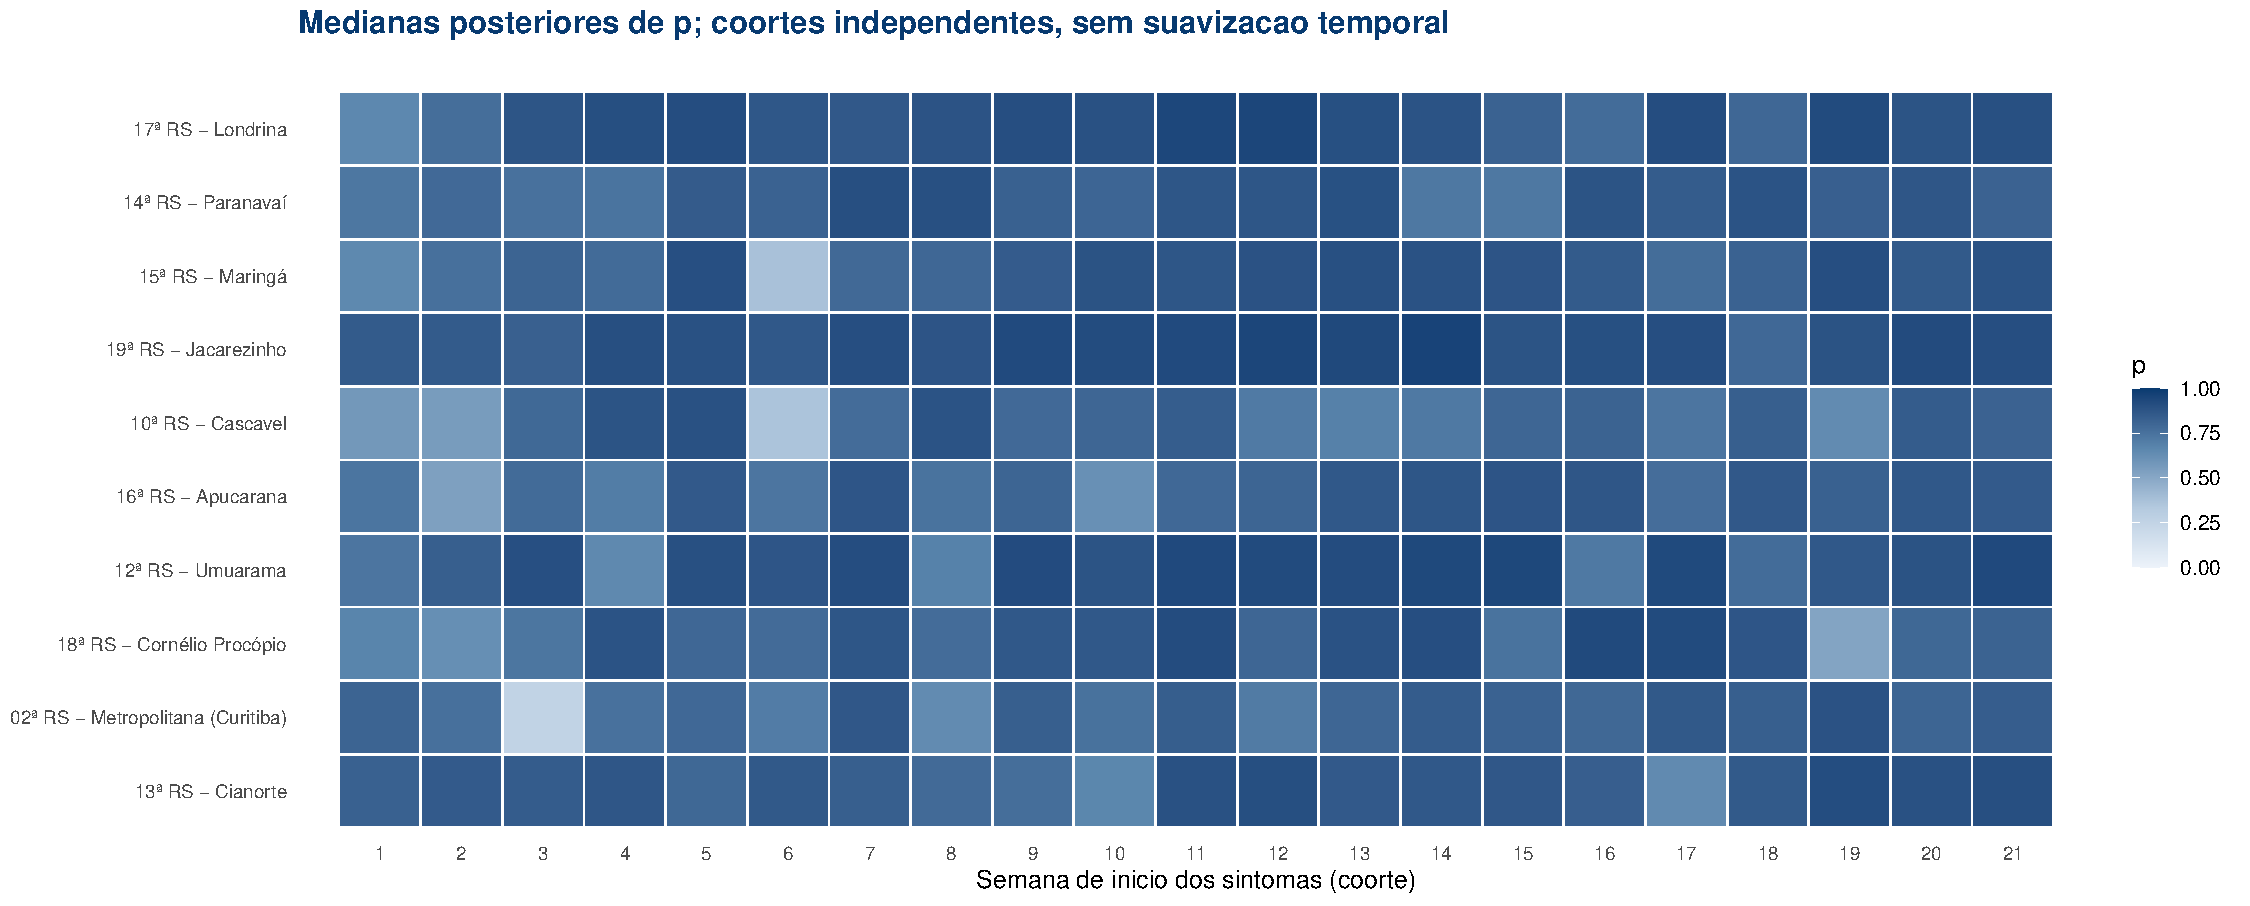
\includegraphics[width=0.95\linewidth]{10D_heatmap_P_COORTES_SEMANAIS.pdf}
\end{center}
\vspace{-12bp}
\begin{center}
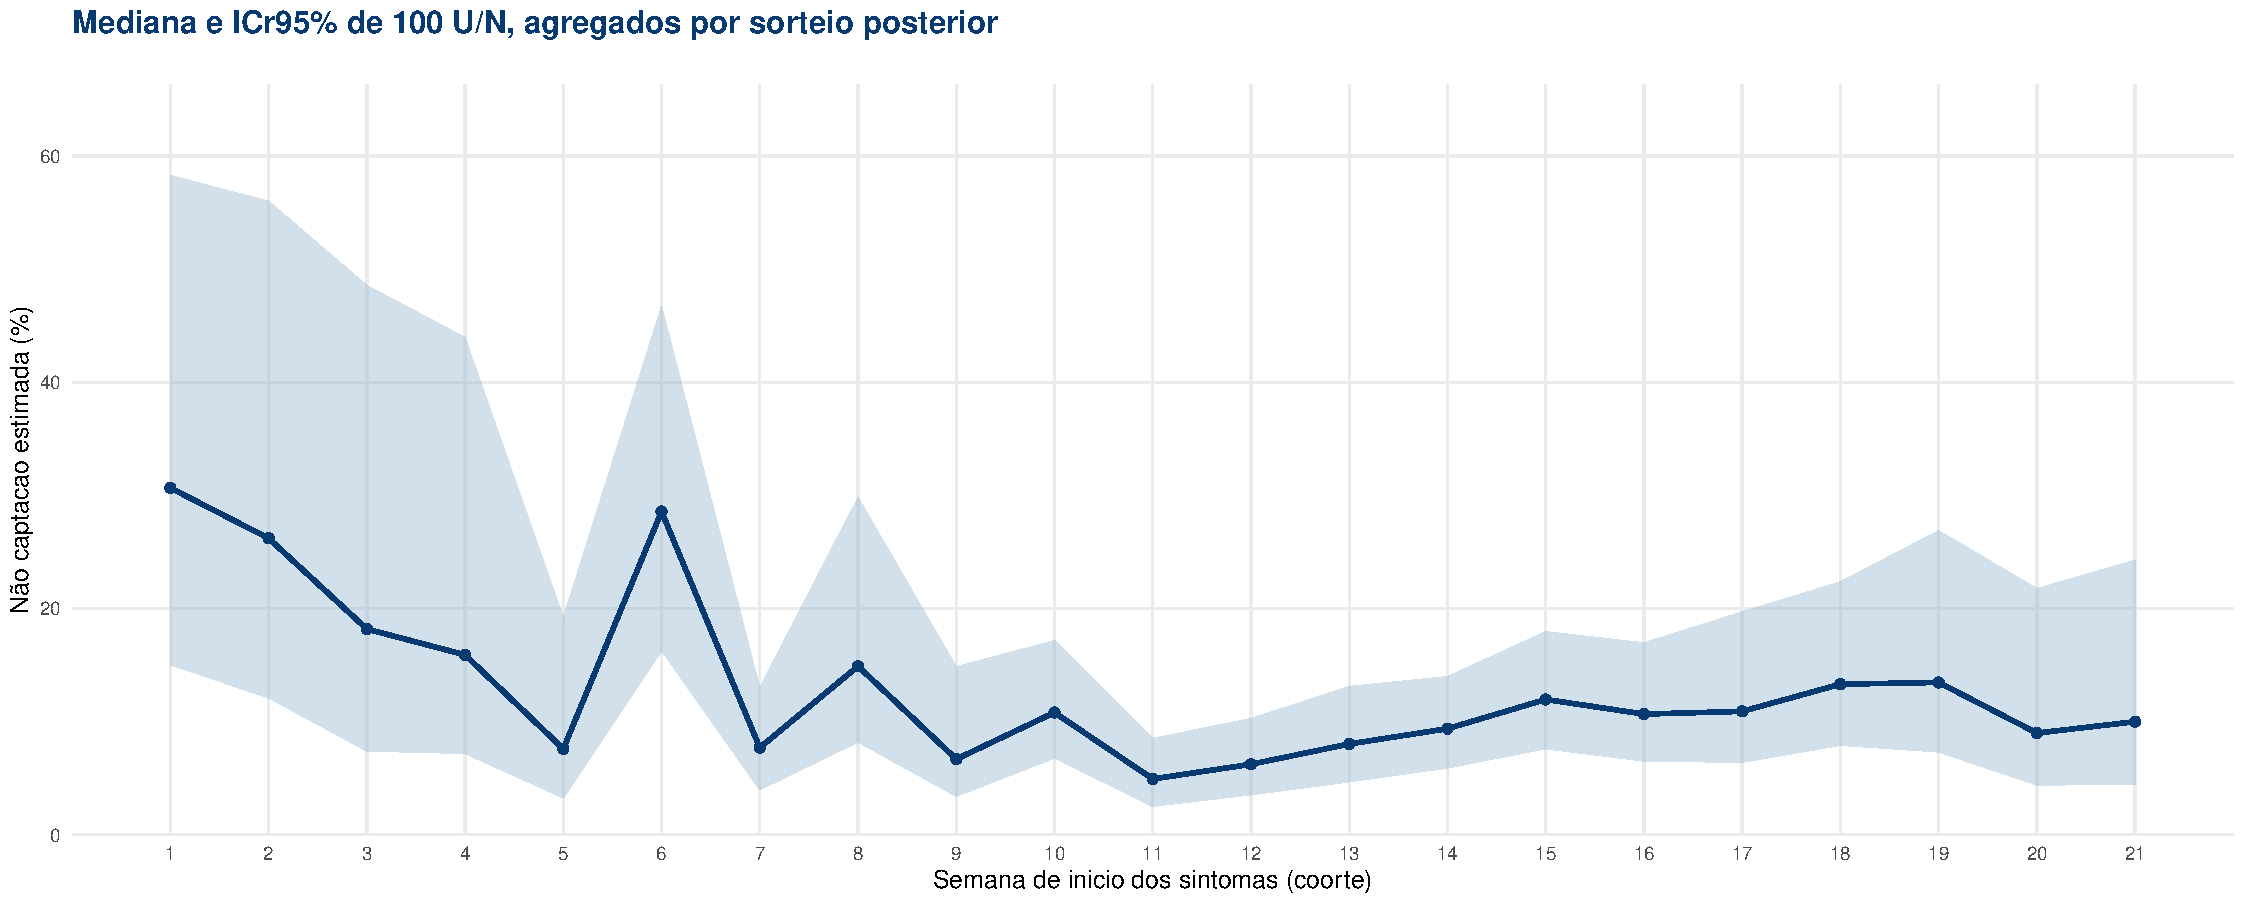
\includegraphics[width=0.95\linewidth]{11A_CURVA_SEMANAL_SUB_TOP10_ICR95.pdf}
\end{center}
{\textoMetodo\color{rbCinza}A linha conecta estimativas de coortes independentes e
não representa suavização temporal. A faixa indica o ICr95\% posterior.\par}

\vspace{53bp}
\tabela{Totais estimados nas 21 coortes das dez RS}
{{\fontsize{23bp}{29bp}\selectfont
\renewcommand\arraystretch{1.15}%
\setlength\aboverulesep{0pt}\setlength\belowrulesep{0pt}%
\begin{tabularx}{\linewidth}{@{}>{\raggedright\arraybackslash}X
  >{\raggedleft\arraybackslash}p{235bp}
  >{\raggedleft\arraybackslash}p{300bp}@{}}
\textbf{Indicador}&\textbf{Mediana}&\textbf{ICr95\%}\\
\arrayrulecolor{rbAzul}\specialrule{3bp}{0pt}{0pt}
\rowcolor{rbFundo}
$C$: notificações observadas & 78.716 & --\\
\arrayrulecolor{rbGrade}\specialrule{1bp}{0pt}{0pt}
$N$: casos latentes & 89.600 & [87.830; 92.097]\\
\arrayrulecolor{rbGrade}\specialrule{1bp}{0pt}{0pt}
$U$: casos não captados & 10.884 & [9.114; 13.381]\\
\specialrule{1bp}{0pt}{0pt}
\rowcolor{rbFundo}
$100U/N$ (\%) & \textbf{12,1} & \textbf{[10,4; 14,5]}\\
\arrayrulecolor{rbAzul}\specialrule{3bp}{0pt}{0pt}
\end{tabularx}}}
{210 ajustes nas dez RS, 21 coortes não sobrepostas; intervalos calculados por sorteio posterior.}

\vspace{32bp}

\tabela{Estimativas posteriores nas dez Regionais de Saúde}
{{\fontsize{15bp}{19bp}\selectfont
\renewcommand\arraystretch{1.04}%
\setlength\tabcolsep{2bp}%
\setlength\aboverulesep{0pt}\setlength\belowrulesep{0pt}%
\begin{tabularx}{\linewidth}{@{}>{\raggedright\arraybackslash}p{190bp}
  *{5}{>{\centering\arraybackslash}X}@{}}
\textbf{Regional} & \textbf{$p$} & \textbf{$\theta$}
& \textbf{$N$} & \textbf{$U$}
& \textbf{$100U/N$ (\%)}\\
\arrayrulecolor{rbAzul}\specialrule{3bp}{0pt}{0pt}
\rowcolor{rbFundo}
17ª Londrina & 0,87 [0,85; 0,89] & 0,50 [0,44; 0,58] & 26.487 [25.968; 27.094] & 2.027 [1.508; 2.634] & 7,7 [5,8; 9,7]\\
\arrayrulecolor{rbGrade}\specialrule{1bp}{0pt}{0pt}
14ª Paranavaí & 0,82 [0,79; 0,84] & 0,49 [0,42; 0,57] & 13.861 [13.444; 14.482] & 1.507 [1.090; 2.128] & 10,9 [8,1; 14,7]\\
\arrayrulecolor{rbGrade}\specialrule{1bp}{0pt}{0pt}
\rowcolor{rbFundo}
15ª Maringá & 0,82 [0,75; 0,85] & 0,60 [0,52; 0,68] & 11.345 [10.873; 12.414] & 1.172 [700; 2.241] & 10,3 [6,4; 18,1]\\
\arrayrulecolor{rbGrade}\specialrule{1bp}{0pt}{0pt}
19ª Jacarezinho & 0,89 [0,84; 0,91] & 0,55 [0,44; 0,66] & 6.908 [6.712; 7.277] & 452 [256; 821] & 6,5 [3,8; 11,3]\\
\arrayrulecolor{rbGrade}\specialrule{1bp}{0pt}{0pt}
\rowcolor{rbFundo}
10ª Cascavel & 0,71 [0,62; 0,77] & 0,35 [0,28; 0,43] & 7.672 [7.107; 8.713] & 1.693 [1.128; 2.734] & 22,1 [15,9; 31,4]\\
\arrayrulecolor{rbGrade}\specialrule{1bp}{0pt}{0pt}
16ª Apucarana & 0,79 [0,69; 0,83] & 0,68 [0,58; 0,77] & 5.423 [5.194; 6.252] & 501 [272; 1.330] & 9,2 [5,2; 21,3]\\
\arrayrulecolor{rbGrade}\specialrule{1bp}{0pt}{0pt}
\rowcolor{rbFundo}
12ª Umuarama & 0,83 [0,70; 0,88] & 0,42 [0,32; 0,54] & 5.660 [5.300; 6.660] & 750 [389; 1.749] & 13,2 [7,3; 26,3]\\
\arrayrulecolor{rbGrade}\specialrule{1bp}{0pt}{0pt}
18ª Cornélio Procópio & 0,78 [0,64; 0,84] & 0,40 [0,30; 0,52] & 5.254 [4.880; 6.415] & 860 [486; 2.021] & 16,4 [10,0; 31,5]\\
\arrayrulecolor{rbGrade}\specialrule{1bp}{0pt}{0pt}
\rowcolor{rbFundo}
02ª Metropolitana & 0,70 [0,52; 0,80] & 0,39 [0,28; 0,51] & 3.322 [2.927; 4.487] & 755 [360; 1.920] & 22,7 [12,3; 42,8]\\
\arrayrulecolor{rbGrade}\specialrule{1bp}{0pt}{0pt}
13ª Cianorte & 0,75 [0,55; 0,84] & 0,38 [0,26; 0,51] & 3.102 [2.762; 4.264] & 602 [262; 1.764] & 19,4 [9,5; 41,4]\\
\arrayrulecolor{rbGrade}\specialrule{1bp}{0pt}{0pt}
\arrayrulecolor{rbAzul}\specialrule{3bp}{0pt}{0pt}
\end{tabularx}}}
{Uma única reprodução MCMC: $p$ e $\theta$ ponderados por $N$;
$N$, $U$ e $100U/N$ agregados por sorteio. ICr95\%: quantis posteriores.}
\end{secao}
\end{colunadireita}
\end{document}